\chapter{Resultados}
\label{chap:res}

A continuación se presentan los resultados detallados de las diferentes versiones del proyecto.

\bigskip

\section{Primera versión}

Tras ejecutar la primera versión, cuya fase de entrenamiento duró \textbf{22.2 segundos}, obtuve los siguientes resultados, formateados en la tabla \ref{tab:v1}. La columna \textit{Época} indica a qué época del entrenamiento hacen referencia los resultados, la columna \textit{Loss} es un valor escalar que intentamos reducir a 0 y la columna \textit{Acierto} indica el porcentaje de aciertos que se han obtenido.

\bigskip

\begin{table}[H]
  \centering
  \begin{tabular}{|l|l|l||l|l|l|}
    \hline
    \textbf{Época} & \textbf{Loss} & \textbf{Acierto} & \textbf{Época} & \textbf{Loss} & \textbf{Acierto} \\
    \hline
    1     & 0.3603 & 0.9007  & 11    & 0.0271 & 0.9927  \\
    2     & 0.1674 & 0.9526  & 12    & 0.0240 & 0.9939  \\
    3     & 0.1205 & 0.9656  & 13    & 0.0209 & 0.9946  \\
    4     & 0.0929 & 0.9736  & 14    & 0.0174 & 0.9958  \\
    5     & 0.0750 & 0.9784  & 15    & 0.0149 & 0.9965  \\
    6     & 0.0622 & 0.9819  &       &        &         \\
    7     & 0.0524 & 0.9853  &       &        &         \\
    8     & 0.0439 & 0.9877  &       &        &         \\
    9     & 0.0375 & 0.9895  &       &        &         \\
    10    & 0.0326 & 0.9911  &       &        &         \\
    \hline
  \end{tabular}
  \label{tab:v1}
  \caption{Resultados de la fase de entrenamiento de la primera versión}
\end{table}

\bigskip

El gráfico \ref{fig:res-v1} refleja los datos de la tabla anterior.

\bigskip

\begin{figure}[H]
  \centering
  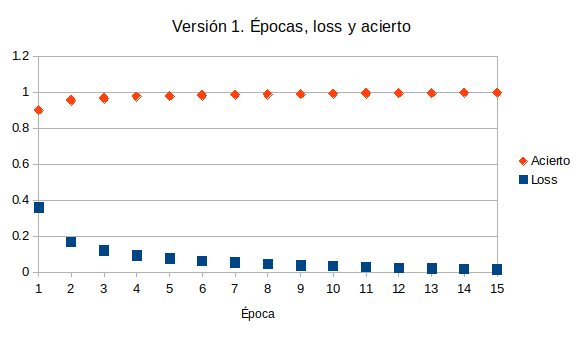
\includegraphics[width=1\textwidth]{../images/results-v1}
  \caption{Gráfico de la fase de entrenamiento de la primera versión}
  \label{fig:res-v1}
\end{figure}

\bigskip

Tras la fase de entrenamiento evalué el modelo, primero con el conjunto de entrenamiento y luego con el conjunto de prueba, y obtuve los siguientes resultados, que pueden verse en la tabla inferior.

\bigskip

\begin{table}[H]
  \centering
  \begin{tabular}{|l|l|l|}
    \hline
    \textbf{Conjunto} & \textbf{Loss} & \textbf{Acierto} \\
    \hline
    Entrenamiento & 0.01141 & 99.80500\%  \\
    Prueba        & 0.07754 & 97.62000\%  \\
    \hline
  \end{tabular}
  \label{tab:results-v1}
  \caption{Resultados de la primera versión dependiendo del conjunto}
\end{table}

\bigskip

A modo de ejemplo, se ha incluido la salida de la consola tras ejecutar esta versión, que puede comprobarse en el  anexo \ref{sec:v1-output}.

\section{Segunda versión}

Tas ejecutar la segunda versión, cuya fase de entrenamiento duró \textbf{309.8 segundos}, obtuve los siguientes resultados.

\bigskip

\begin{table}[H]
  \centering
  \begin{tabular}{|l|l|l||l|l|l|}
    \hline
    \textbf{Época} & \textbf{Loss} & \textbf{Acierto} & \textbf{Época} & \textbf{Loss} & \textbf{Acierto} \\
    \hline
    1                       & 0.3648 & 0.8989 & 11 & 0.0497 & 0.9845 \\
    2                       & 0.1361 & 0.9618 & 12 & 0.0478 & 0.9854 \\
    3                       & 0.1361 & 0.9712 & 13 & 0.0455 & 0.9860 \\
    4                       & 0.0847 & 0.9757 & 14 & 0.0410 & 0.9872 \\
    5                       & 0.0759 & 0.9773 & 15 & 0.0404 & 0.9874 \\
    6                       & 0.0691 & 0.9791 &    &        &        \\
    7                       & 0.0628 & 0.9815 &    &        &        \\
    8                       & 0.0599 & 0.9821 &    &        &        \\
    9                       & 0.0567 & 0.9830 &    &        &        \\
    10                      & 0.0522 & 0.9835 &    &        &        \\
    \hline
  \end{tabular}
  \label{tab:v2}
  \caption{Resultados de la fase de entrenamiento de la segunda versión}
\end{table}

\bigskip

El gráfico \ref{fig:res-v2} refleja los datos de la esta tabla.

\bigskip

\begin{figure}[H]
  \centering
  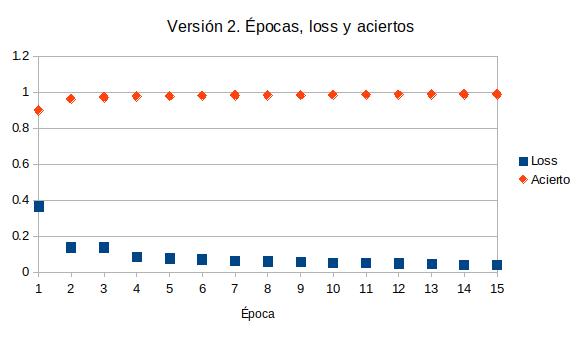
\includegraphics[width=1\textwidth]{../images/results-v2}
  \caption{Gráfico de la fase de entrenamiento de la segunda versión}
  \label{fig:res-v2}
\end{figure}

\bigskip

Tras la fase de entrenamiento evalué el modelo, primero con el conjunto de entrenamiento y luego con el conjunto de prueba, y obtuve los siguientes resultados.

\bigskip

\begin{table}[H]
  \centering
  \begin{tabular}{|l|l|l|}
    \hline
    \textbf{Conjunto} & \textbf{Loss} & \textbf{Acierto} \\
    \hline
    Entrenamiento & 0.02590 & 99.27000\%  \\
    Prueba        & 0.05184 & 98.22000\%  \\
    \hline
  \end{tabular}
  \label{tab:results-v2}
  \caption{Resultados de la segunda versión dependiendo del conjunto}
\end{table}

\bigskip

\section{Tercera versión}

Tas ejecutar la tercera versión, cuya fase de entrenamiento duró 309.8 segundos, obtuve los siguientes resultados.

\bigskip

\begin{table}[H]
  \centering
  \begin{tabular}{|l|l|l||l|l|l|}
    \hline
    \textbf{Época} & \textbf{Loss} & \textbf{Acierto} & \textbf{Época} & \textbf{Loss} & \textbf{Acierto} \\
    \hline
    1                       & 0.1970 & 0.9389 & 11 & 0.0093 & 0.9971 \\
    2                       & 0.0560 & 0.9831 & 12 & 0.0088 & 0.9973 \\
    3                       & 0.0385 & 0.9882 & 13 & 0.0074 & 0.9978 \\
    4                       & 0.0288 & 0.9909 & 14 & 0.0078 & 0.9975 \\
    5                       & 0.0227 & 0.9934 & 15 & 0.0055 & 0.9983 \\
    6                       & 0.0198 & 0.9940 & 16 & 0.0076 & 0.9977 \\
    7                       & 0.0160 & 0.9952 & 17 & 0.0060 & 0.9983 \\
    8                       & 0.0130 & 0.9957 & 18 & 0.0064 & 0.9980 \\
    9                       & 0.0114 & 0.9964 & 19 & 0.0039 & 0.9988 \\
    \hline
  \end{tabular}
  \label{tab:v3}
  \caption{Resultados de la fase de entrenamiento de la tercera versión}
\end{table}

\bigskip

El gráfico \ref{fig:res-v3} refleja los datos de la esta tabla.

\bigskip

Tras la fase de entrenamiento evalué el modelo, primero con el conjunto de entrenamiento y luego con el conjunto de prueba, y obtuve los siguientes resultados.

\bigskip

\begin{table}[H]
  \centering
  \begin{tabular}{|l|l|l|}
    \hline
    \textbf{Conjunto} & \textbf{Loss} & \textbf{Acierto} \\
    \hline
    Entrenamiento & 0.00237 & 99.90167\%  \\
    Prueba        & 0.04271 & 99.15000\%  \\
    \hline
  \end{tabular}
  \label{tab:results-v3}
  \caption{Resultados de la tercera versión dependiendo del conjunto}
\end{table}

\bigskip

\begin{figure}[H]
  \centering
  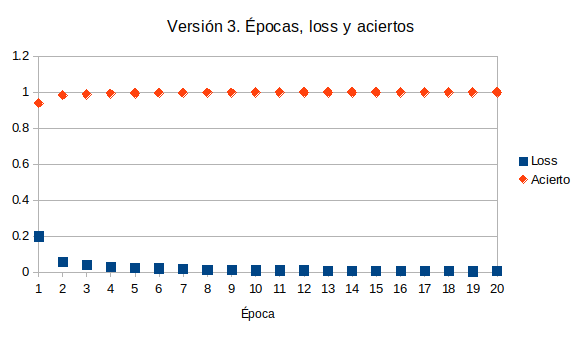
\includegraphics[width=1\textwidth]{../images/results-v3}
  \caption{Gráfico de la fase de entrenamiento de la tercera versión}
  \label{fig:res-v3}
\end{figure}

\bigskip

Por lo tanto, el \textbf{resultado final} del proyecto sobre el conjunto de prueba es de un 99.15\%, lo que supone tan solo un \textbf{0.85\% de fallos sobre los 10,000 números manuscritos}, o lo que es lo mismo, 85 errores.
